\documentclass[12pt, a4paper]{article}
\usepackage[utf8]{inputenc}
\usepackage[left=2cm,right=2cm,top=1.5cm,bottom=1.5cm]{geometry}
\usepackage{xcolor}
\usepackage{tikz}
\usetikzlibrary{arrows.meta, positioning, patterns, patterns.meta}
\usepackage{amsmath}
\usepackage{amsthm}
\usepackage{amssymb}
\usepackage{pgfplots}
\usepackage{rotating}
\usepackage{pgfmath}
\usepackage{multicol}

%---------------------------------------------
\begin{document}
\begin{multicols}{2}
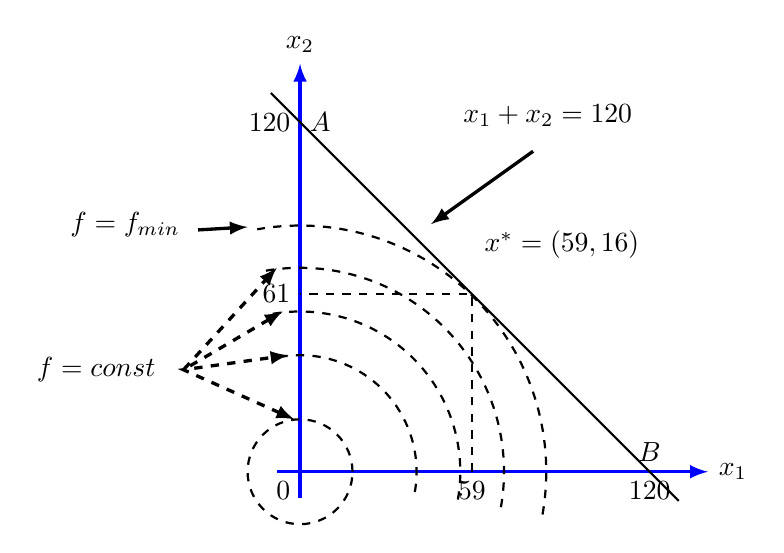
\begin{tikzpicture}[scale=0.037]
\draw[-latex,very thick, blue](-8,0) -- (140,0) node[right, black]{$x_1$};\\
\draw[-latex,very thick, blue](0,-9) -- (0,140) node[above, black]{$x_2$};
\draw[thick] (-10,130) -- (130, -10);
\node[below left] at (0,0) {0};
\node[right] at (0,120) {$A$};
\node[left] at (0,120) {120};
\node[above] at (120,0)  {$B$};
\node[below] at (120,0)  {120};
\node[above] at (85,115) {$x_1+x_2=120$};
\draw[-latex,very thick] (80,110)--(45,85);
\node[above right] at(60,70) {$x^{*}=(59,16)$};
\node[below] at(59, 0) {59};
\node[left] at (0,61) {61};
\draw[dashed, thick] (59,0) -- (59,61) -- (0,61);
\draw[thick, dashed] (0,0) circle (18);
\foreach \i in {40,55,70,84.5}{
\draw[thick, dashed] (0,0)+(-10:\i) arc[start angle = -10, end angle = 100, radius = \i];
};
\node at (-70,35) {$f = const$};
\draw[latex-latex, very thick, dashed] (-2,18) -- (-40,35) -- (-4,40);
\draw[latex-latex, very thick, dashed] (-6,55) -- (-40,35) -- (-8,70);
\node at (-60, 85)  {$f = f_{min}$};
\draw[-latex, very thick] (-35,83) -- (-18, 84);
\end{tikzpicture}
\hspace{2cm}


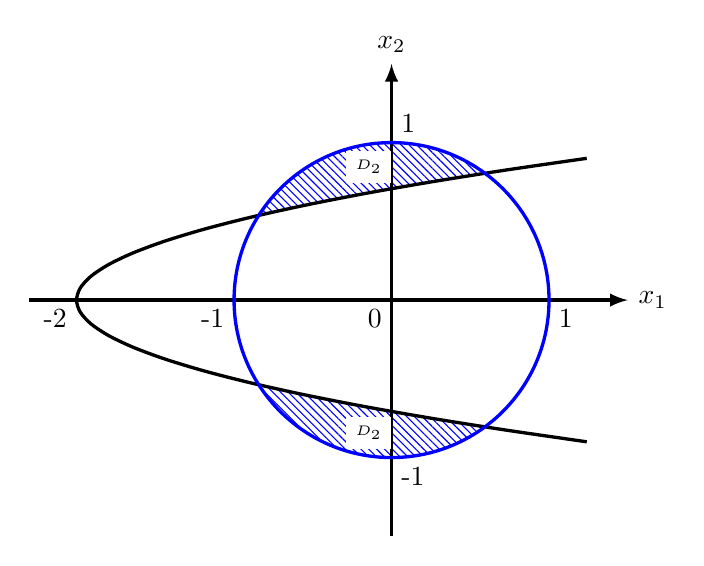
\begin{tikzpicture}[scale = 2]
\fill[pattern = {Lines[angle = -45, distance = 2pt]}, pattern color = blue] (0,0) circle (1);
\draw[fill = white, very thick] plot[smooth,domain = -0.9:0.9] ({\x*\x*4 - 2}, \x);
\draw[very thick, -latex] (-2.3,0) -- (1.5,0) node[right]{$x_1$};
\draw[very thick, -latex] (0, -1.5) -- (0, 1.5) node[above]{$x_2$};
\foreach \i in {-2,-1}
\node[below left] at (\i, 0) {\i};
\node[below right] at(1,0){1};
\node[above right] at (0,1) {1};
\node [below right] at(0,-1) {-1};
\node[below left] at (0,0) {0};
\draw[very thick, blue] (0,0) circle (1);
\node[fill = white, below left] at (0,0.95) {\tiny{$D_2$}}; 
\node[fill = white, above left] at (0,-0.95) {\tiny{$D_2$}}; 
\end{tikzpicture}
\end{multicols}



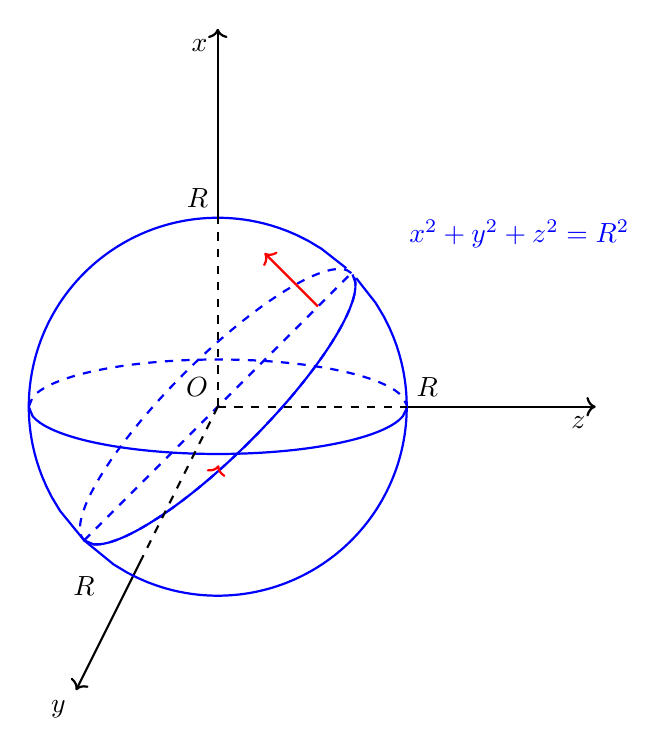
\begin{tikzpicture}[scale=1.2]
\draw[thick,->](0,2)--(0,4)node[anchor=north east]{$x$};
\draw[thick,->](-0.8,-1.6)--(-1.5,-3)node[anchor=north east]{$y$};
\draw[thick,->](2,0)--(4,0)node[anchor=north east]{$z$};
\begin{scope}[rotate=45,xshift=0cm,yshift=-2cm]
\draw[blue,thick,domain=-2:2,samples=100] plot ({\x},{2+sqrt(4-(\x)^2)});
\draw[blue,thick,domain=-2:2,samples=100] plot ({\x},{2-sqrt(4-(\x)^2)});
\draw[thick,blue,dashed] (0,2) ellipse (2 and 0.5);
\draw[blue,thick,domain=-2:2,samples=100] plot ({\x},{-0.5*sqrt(1-(\x)^2/4)+2});
\draw[thick,dashed, blue](-2,2)--(2,2); 
\draw[thick, red, ->](1.5,2)--(1.5,2.8); 
\end{scope}
\draw[blue,thick,dashed,domain=-2:2,samples=100] plot ({\x},{0.5*sqrt(1-(\x)^2/4)});
\draw[blue,thick,domain=-2:2,samples=100] plot ({\x},{-0.5*sqrt(1-(\x)^2/4)});
\draw[thick,dashed](0,0)--(0,3); 
\draw[thick,dashed](0,0)--(2,0); 
% \draw[thick](-4,0)--(-2,0); 
\draw[thick,dashed](0,0)--(-0.8,-1.6); 
\draw[->,thick, red](0,-0.65)--(0.01,-0.62);
\node [above left] at (0,0) {$O$};
\node [above left] at (0,2) {$R$};
\node [above right] at (2,0) {$R$};
\node [above left] at (-1.2,-2.1) {$R$};
\draw (2,2) node [anchor=north west][inner sep=0.75pt]   [align=left] {\textcolor[rgb]{0.00,0.00,1.00}{$x^2+y^2+z^2=R^2$}};
\end{tikzpicture}
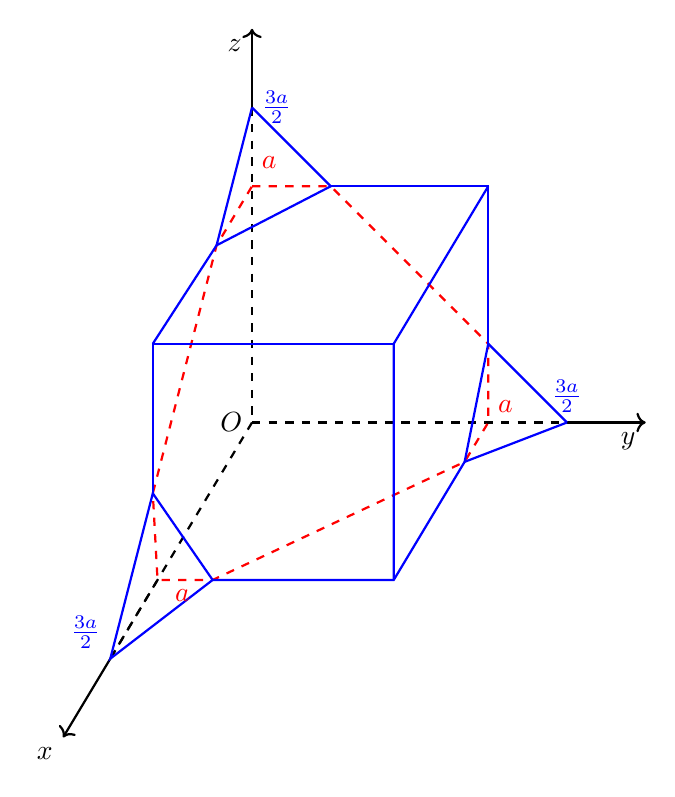
\begin{tikzpicture}
% \draw[help lines, dashed, red] (-5,-5) grid (5,5);
\draw[thick,->](4,0)--(5,0)node[anchor=north east]{$y$};
\draw[thick,->](0,4)--(0,5)node[anchor=north east, dashed]{$z$};
\draw[thick,->](-1.8,-3)--(-2.4,-4)node[anchor=north east]{$x$};
\draw[thick, dashed](0,4)--(0,0);
\draw[thick, dashed](0,0)--(4,0);
\draw[thick, dashed](0,0)--(-1.8,-3);
\draw[thick, dashed](-1.8,-3)--(-1.2,-2);
\draw[ thick, dashed, red](0,3)--(1,3)--(3,1)--(3,0)--(2.7,-0.5)--(-0.5,-2)--(-1.2,-2)--(-1.26,-0.9)--(-0.45,2.25)--(0,3);
\draw[thick, blue](1,3)--(3,3)--(3,1);
\draw[thick, blue](-0.45,2.25)--(-1.26,1);
\draw[thick, blue](-1.8,-3)--(-1.26,-0.9)--(-0.5,-2)--cycle;
\draw[thick, blue](2.7,-0.5)--(1.8,-2)--(-0.5,-2);
\draw[thick, blue](0,4)--(1,3)--(-0.45,2.25)--(0,4);
\draw[thick, blue](4,0)--(3,1)--(2.7,-0.5)--(4,0);
\draw[thick, blue](1.8,-2)--(1.8,1)--(3,3);
\draw[thick, blue](1.8,1)--(-1.26,1)--(-1.26,-0.9);
\node[left, black] at (0,0){$O$};
\node[right, blue] at (0,4) {$\frac{3a}{2}$};
\node[above, blue] at (4,0) {$\frac{3a}{2}$};
\node[above left, blue] at (-1.8,-3){$\frac{3a}{2}$};
\node[above right, red] at (3,0) {$a$};
\node[right, red] at (0,3.3) {$a$};
\node[right, red] at (-1.1,-2.2) {$a$};
\end{tikzpicture}


\end{document}